\subsection{Case04 - Layer 3 forwarding}
\label{p4_wifi_case04}


 En este caso de uso trataremos de implementar un forwarding a nivel de red, capa 3, por ello nuestro hipotético "switch" será ahora un un router muy básico y con muy pocas funcionalidades. Al igual que en los casos de uso anteriores, se hará uso de software switch llamado \gls{bmv2}, para testear los programas P4, y de la integración desarrollada anteriormente con Mininet-WiFi como escenario para recrear las topologías de Red. En este caso también, el \gls{bmv2} será configurado vía P4Runtime  por lo que se hará uso de la clase de \texttt{P4RuntimeAP}. En el caso de querer configurar el \gls{bmv2} vía Thrift-port se podría utilizar la clase desarrollada \texttt{P4AP}.\\
\par

Dado que toda la información relativa a este caso de uso ya se ha explicado anteriormente en el case04 de P4 cableado (Ver subsección \ref{P4_ether_case04}), y no hay ninguna diferencia inducida en el cambio de entorno según se explico en las sección anterior,  únicamente se harán indicaciones sobre como poder compilarlo y ejecutarlo. Importante, si usted está replicando este caso de uso, sin antes haber adecuado las dependencias necesarias de Mininet-WiFi con soporte del \gls{bmv2}, vuelva a este punto \ref{mn_wifi_own_deps} y siga los pasos indicados.\\
\par

% figura escenario
\begin{figure}[ht]
    \centering
    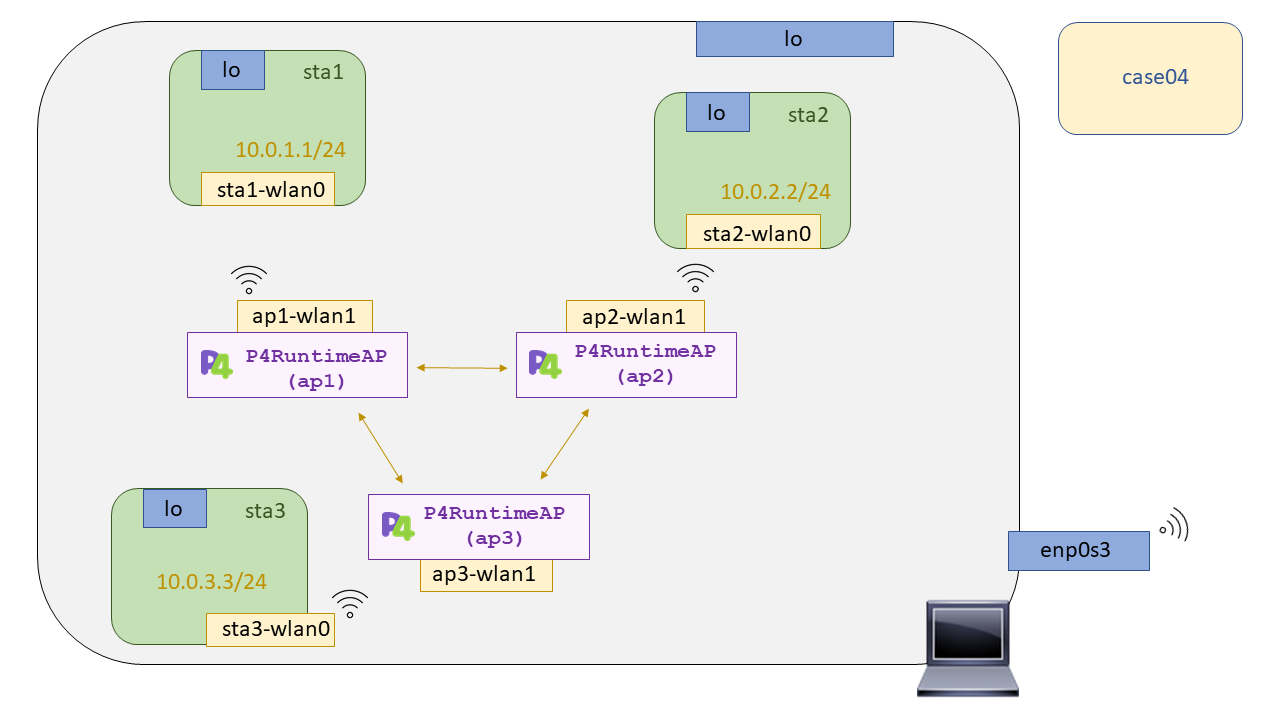
\includegraphics[width=16cm]{archivos/img/dev/p4-wifi/case04/scenario.png}
    \caption{Escenario del Case04 - P4 Wireless}
    \label{fig:case04_p4_wifi_scenario}
\end{figure}



\vspace{0cm}
\textbf{Compilación}\\
\par

Para la compilación de este caso de uso, al igual que en los casos de uso anteriores se ha dejado preparado un Makefile, por tanto no es necesario que el usuario haga un uso directo del compilador p4c. Si se quiere saber más sobre como funciona el proceso de compilación, qué etapas hay, como se le "inyecta" el \texttt{json} generado al \gls{bmv2}, o qué distintos \textit{targets} hay en función de la arquitectura, le recomendamos que vuelva al case01 (\ref{p4_ether_case01}). Para llevar a cabo la compilación solo se tendrá que seguir los pasos indicados en el bloque \ref{code:case04_p4_wifi_load}.

\begin{lstlisting}[language= bash, style=Consola, caption={Compilación programa P4  - Case04},label=code:case04_p4_wifi_load]
    # Entramos al directorio 
    cd TFG/src/use_cases/p4-wireless/case04

    # Hacemos uso del Makefile
    sudo make
\end{lstlisting}
\vspace{0.5cm}


Una vez ejecutado el make, se habrá generado una estructura de directorios que se utilizarán en el lanzamiento del caso de uso. Bajo el directorio \texttt{build} se podrá encontrar el \texttt{json} generado por el compilador, será este \texttt{json} quien tenga toda la información requerida para conformar el \gls{bmv2}. Los directorios \texttt{log} y \texttt{pcap}, se utilizarán respectivamente para almacenar los logs del \gls{bmv2} y para guardar las capturas de paquetes de las interfaces asociadas a la instancia \gls{bmv2}. Comentar que la interfaz desarrollada admite opciones para no generar información de log, ni pcaps, se podrá configurar a medida desde el propio script que lanza el escenario.\\
\par



\vspace{0.2cm}
\textbf{Puesta en marcha del escenario}\\
\par

Al igual que en la compilación, se ha dejado preparado un script en Python para automatizar la puesta en marcha del escenario. Este script describe la topología que se utilizará en este caso de uso. Recordar que es necesario volver hacer un \texttt{make install} para instalar los módulos adicionales generados para la integración del \gls{bmv2} y Mininet-WiFi, además de tener instaladas las versiones indicadas en el análisis de la integración. Estas dependencias se pueden encontrar en el apartado \ref{mn_wifi_own_deps}. Una vez comprobado que posee todas la dependencias, simplemente se tendrá que ejecutar el script con el interprete de Python. Este script levantará la topología descrita en la figura \ref{fig:case04_p4_wifi_scenario}, compuesto por tres estaciones WiFi y por tres instancias del nodo \texttt{P4RuntimeAP}. Los nodos \texttt{apX}, del tipo \texttt{P4RuntimeAP}, tendrán tres interfaces, una wireless y dos par de \gls{veth} para comunicarse entre los distintos puntos de acceso.


\begin{lstlisting}[language= bash, style=Consola, caption={Puesta en marcha del escenario  - Case04},label=code:case04_p4_wifi_run]
    sudo python scenario.py
\end{lstlisting}


\vspace{0.5cm}
\textbf{Comprobación del funcionamiento}\\
\par


Tras las ejecución del script \texttt{scenario.py}, se tendría el escenario \ref{fig:case04_p4_wifi_scenario} levantado, y la CLI de Mininet-WiFi abierta. Para la comprobación de funcionamiento de este caso de uso, se van a seguir los mismos pasos que en el case05 (\ref{P4_ether_case05}) - P4 en un entorno alámbrico. Por tanto no se entrará hacer explicaciones que se creen redundantes, se indicarán los pasos seguidos para llevar a cabo la comprobación de funcionamiento y los resultados de dichas pruebas. 

\begin{lstlisting}[language= bash, style=Consola, caption={Pasos a seguir para comprobar el funcionamiento - Case04},label=code:case04_p4_wifi_func1]
    mininet-wifi>  pingall
\end{lstlisting}
\vspace{0.5cm}


% figura escenario
\begin{figure}[ht]
    \centering
    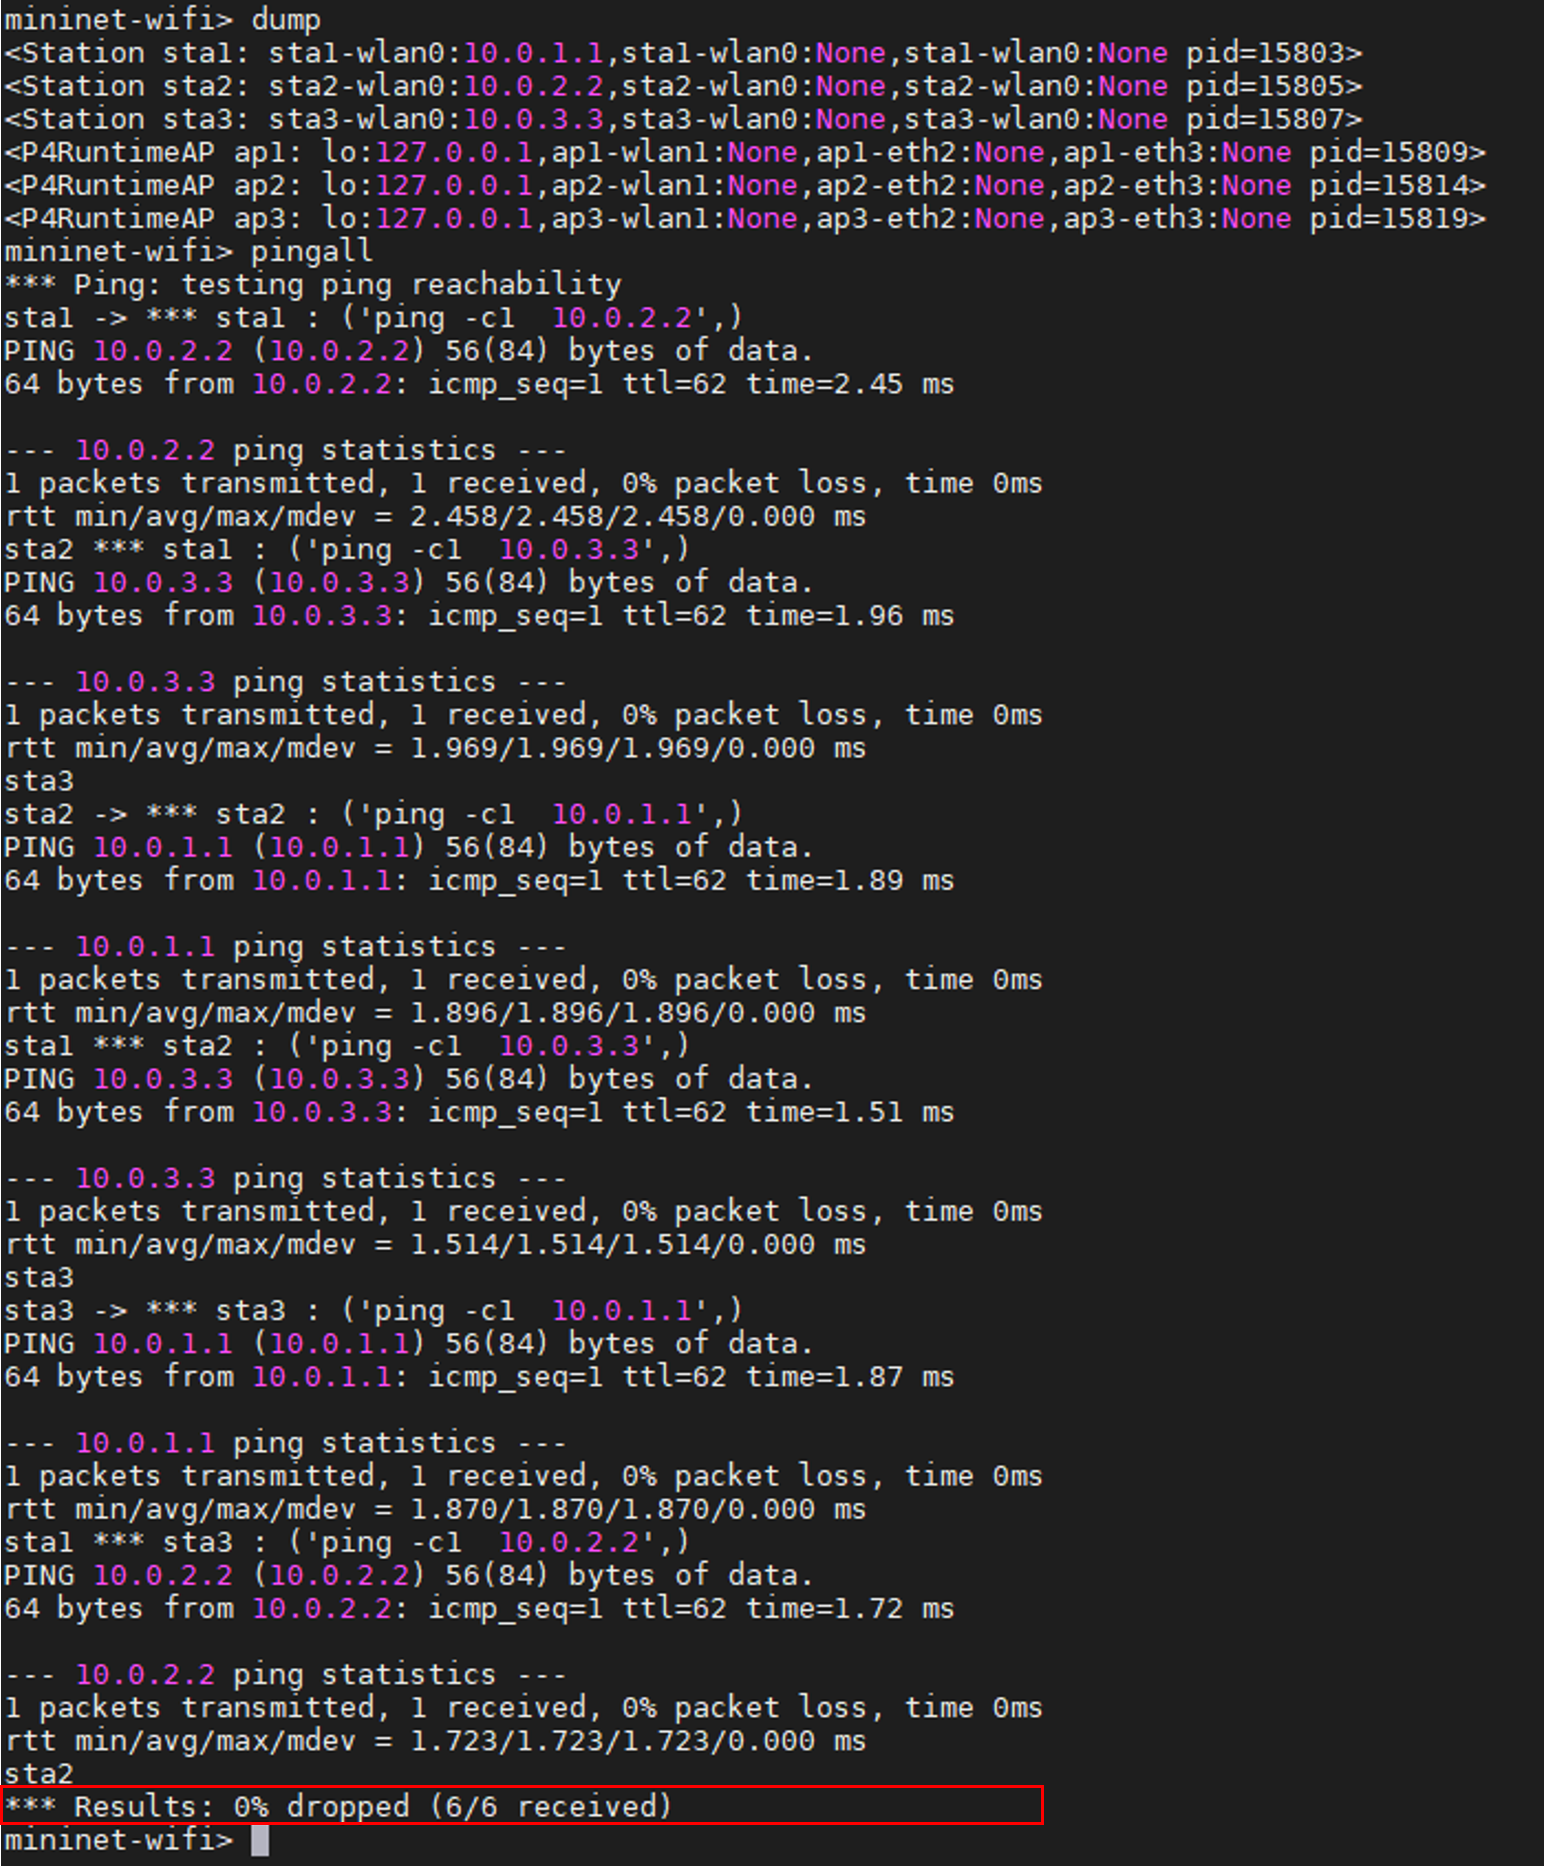
\includegraphics[width=10cm]{archivos/img/dev/p4-wifi/case04/demo_case04_edited.png}
    \caption{Comprobación de funcionamiento del Case04 - P4 Wireless}
    \label{fig:case04_p4_wifi_func1}
\end{figure}


Según se puede apreciar en la figura \ref{fig:case04_p4_wifi_func1}, hay perfecta conectividad entre todos los hosts de la topología. Además, se podría hacer uso de un \textit{sniffer} para comprobar que los paquetes llegan con el campo \texttt{ttl} modificado, en función de los saltos que ha dado el paquete. 